\documentclass[12pt]{article}
\usepackage[utf8]{inputenc}
\usepackage[T1]{fontenc}
\usepackage{hyperref}
\usepackage{lipsum} % for placeholder text, remove if not needed
\usepackage[a4paper, portrait, margin=1.5cm]{geometry}
\usepackage{graphicx}
\usepackage{fancyhdr}
\usepackage{float}
\usepackage{color}
\usepackage{subcaption}
\usepackage{parskip}
\definecolor{orange}{rgb}{1,0.5,0}


\title{\textbf{A mobile application for augmenting technical documentation using AR and AI}}
\author{Ani Bitri\\ \small Dr. Paris Giampouras, John McNamara\\ \small University of Warwick and IBM}



\begin{document}
\begin{figure}
    \centering
    \begin{subfigure}[b]{0.45\textwidth}
        \centering
        
\includegraphics[height=4cm]{img/WarwickCrest.png}
        \label{fig:WarwickCrest}
    \end{subfigure}
    \hfill
    \begin{subfigure}[b]{0.45\textwidth}
        \centering
        
\includegraphics[height=4cm]{img/IBM_Logo.png}
        \label{fig:IBM_Logo}
    \end{subfigure}
\end{figure}

\date{October 2025}
\maketitle

\newpage

\section{Problem Statement}

    \subsection{Introduction and Context}

        Technical documentation plays a critical role in helping developers understand, implement, operate and maintain software systems. In enterprise environments, documentation is the primary interface between developers and complex
        systems, making clarity and accessibility essential. However, despite its importance, technical documentation remains predominantly static, text-based and difficult to navigate. As systems grow in complexity, dynamic processes such
        as data flows, dependencies and interactions are often poorly represented in traditional documentation formats. Consequently, many users often struggle to find the information they need, leading to frustration, errors and inefficiencies. This 
        raises the need for innovative solutions that can enhance the user experience and improve comprehension of technical documentation.

    \subsection{Existing Technologies}

    There are several existing technologies which address parts of the problem but do not yet offer a comprehensive solution. These include:
        \begin{itemize}
            \item \textbf{Static and Web-Based Documentation:}
                Different Platforms like GitBook, ReadTheDocs and Markdown-based tools offer well-structured and accessible documentation but lack interactivity and visualization capabilities. Information is conveyed effectively through text and images
                but remains static and fails to envision the dynamic nature of modern software systems.
            \item \textbf{AI Assistants:}
                In the last few years, the rise of AI-powered assistants like ChatGPT and Gemini have been transformative. These tools can understand and interpret technical text, summarize content and answer user queries. Yet, these
                assistants operate in isolation from the documentation itself, requiring users to switch contexts and manually input queries, disconnecting them from visual elements and offering limited support for the understanding of
                system architecture and interactions.
            \item \textbf{Augmented Reality Applications:}
                Industrial AR tools, such as PTC Vuforia, Microsoft Dynamics 365 Guides and Scope AR, have been used to overlay digital information onto real-world objects. These solutions enhance spatial understanding and are particularly useful in maintenance
                and training contexts. However, they typically rely on specific and expensive hardware, such as the HoloLens, or complex 3D models, thus limiting their accessibility for general users.
        \end{itemize}

    \subsection{Gaps in Current Solutions}

        Despite the advancements in AR and AI technologies, the current solutions exhibit several limitations:
        \begin{itemize}
            \item \textbf{Lack of Integration between AR and AI:}
                Visualization (AR) and comprehension (AI) are treated as separate domains. There is limited integration or implementation that combines the strengths of both to deliver a seamless user experience.
            \item \textbf{Limited Visual Comprehension:}
                Text and 2D diagrams are insufficient for conveying complex interactions and dynamic processes. Current documentation formats do not effectively utilize visual aids to enhance understanding.
            \item \textbf{Hardware and Platform Barriers:}
                Most AR implementations are dependent on specialized hardware, such as the HoloLens or AR glasses, which are costly or not widely available. This restricts the accessibility of AR-enhanced documentation to a broader audience.
        \end{itemize}

    \subsection{Problem Definition}

    Given the limitations of existing documentation systems and the potential of emerging technologies, there is a need for an innovative solution which can be easily accessible, interactive and capable of enhancing
    the understanding of technical documentation. In order to address this need, the project aims to develop an AI-powered mobile application that uses AR technology to augment technical documentation. The proposed system must 
    allow users to point their mobile devices at a technical diagram and view interactive AR overlays that explain components, relationships and interactions. At the same time, an integrated AI assistant, IBM Watson/Granite,
    will be available to answer user queries and provide additional context. Therefore, this project aims to bridge the gap between visual comprehension and intelligent interaction in technical documentation, ultimately demonstrating how static documents can become interactive, explainable and user-friendly.


\section{Project Overview}

    \subsection{Purpose}
    This project aims to create an AI-powered mobile application which, supported by AR technology, will enhance the user experience
    by providing interactive and immersive documentation. Powered by IBM Watson/Granite, the app will offer several features to assist developers in navigating and comprehending complex technical documents, including text recognition,
    interactive AR overlays, chatbot assistance and more.

    \subsection{Objectives within the scope}
    The primary objectives of this project are to:
    \begin{enumerate}
        \item Implement AR diagram augmentation
        \begin{itemize}
            \item Detect and track diagrams in printed and digital forms.
            \item Overlay interactive elements on diagrams to provide additional context and explanations.
        \end{itemize}
        \item Integrate an AI assistant
        \begin{itemize}
            	\item Employ IBM Watson/Granite to interpret the scanned documentation text and answer user queries.
            	\item Support natural language questions such as "What is the purpose of this diagram?" or "Explain this concept in simpler terms.".
        \end{itemize}
    \item Preserve accessibility and compliance
        \begin{itemize}
            \item Keep the core document unchanged and externalize enhancements through AR overlays to comply with accessibility and legal requirements.
        \end{itemize}
        \item Develop a functional mobile prototype
        \begin{itemize}
            \item Deliver a working mobile application prototype that demonstrates the key features and functionalities.
            \item Conduct user testing to gather feedback and refine the application.
            \item Provide a short demonstration.
        \end{itemize}
        \end{enumerate}

    \subsection{Boundaries and Out-of-Scope Elements}
    To keep the project achievable within the given timeframe, the following elements are considered out of scope:
    \begin{itemize}
        \item Full production deployment or enterprise-level integration.
        \item Hardware-specific AR is excluded; the focus is on mobile devices.
        \item Cross-platform optimization beyond the primary target platform (e.g., iOS or Android).
    \end{itemize}

    \subsection{Expected Deliverables}
    \begin{itemize}
        \item A prototype mobile application demonstrating real-time recognition and overlay of technical documentation.
        \item Integrated AI assistant interface capable of answering user queries based on the documentation content.
        \item A comprehensive project report detailing the design, implementation, testing processes and evaluation results.
        \item VIVA presentation and demonstration.
    \end{itemize}

    \subsection{Target Outcomes}
    \begin{itemize}
        \item Enhanced user experience for developers interacting with technical documentation.
        \item Improved comprehension of complex technical concepts through interactive AR elements and AI assistance.
        \item A foundation for future development and potential commercialization of the application.
    \end{itemize}




\section{Methods and Methodologies}
    \subsection{Development Methodology}
    Given the dynamic nature of the project and the need for iterative development, the Scrum framework within the Agile methodologies will be adopted. The approach will allow for flexibility, continuous feedback
    and incremental delivery of features. Weekly stand-up meetings will be held to discuss progress and address any challenges. The work will be organized into sprints, each lasting approximately one to two weeks,
    with clearly defined goals. At the end of each sprint, a review session will be held with the assessors to demonstrate progress and gather feedback.
    
    \subsection{Version Control and Documentation}
    Version control will be managed using Git and GitHub, ensuring all changes are tracked and documented. Regular commits will be made to maintain a history of the development process. This
    approach supports the Scrum framework by ensuring transparency, traceability and code integrity throughout the project lifecycle.

    \subsection{Requirement Gathering and Analysis}
    Requirements will be gathered and refined through continuous engagement with the assessors, ensuring the project remains aligned with the initial objectives. Any changes to the requirements will be documented and communicated promptly.
    Research into existing technologies and best practices will be conducted to inform design decisions and implementation strategies. This includes exploring AR frameworks, AI integration techniques and mobile development tools.

    \subsection{Testing and Evaluation}

    In order to have an objective and reliable evaluation of the application, a series of tests will be conducted throughout the development process. These tests will ensure the functionality, usability and performance of the application. Moreover, user testing will be performed with a
    small group of target users to gather feedback and identify areas for improvement. The testing process will include:
        \begin{itemize}
            \item \textbf{Unit Testing:} Individual components and functions will be tested to ensure they work as intended.
            \item \textbf{Integration Testing:} The interaction between different components, such as AR overlays and AI responses, will be tested to ensure seamless functionality.
            \item \textbf{User Acceptance Testing (UAT):} Target users will test the application to provide feedback on usability, functionality and overall experience.
            \item \textbf{Performance Testing:} The application will be evaluated for responsiveness, load times and resource usage to ensure optimal performance on mobile devices.
        \end{itemize}

    \subsection{Time Management and Milestones}
        The Gantt chart below outlines the planned work schedule, including key milestones and deadlines. Weekly meetings with the assessors will also be scheduled to ensure alignment and address any issues promptly. 
        \begin{figure}[H]
        \centering
        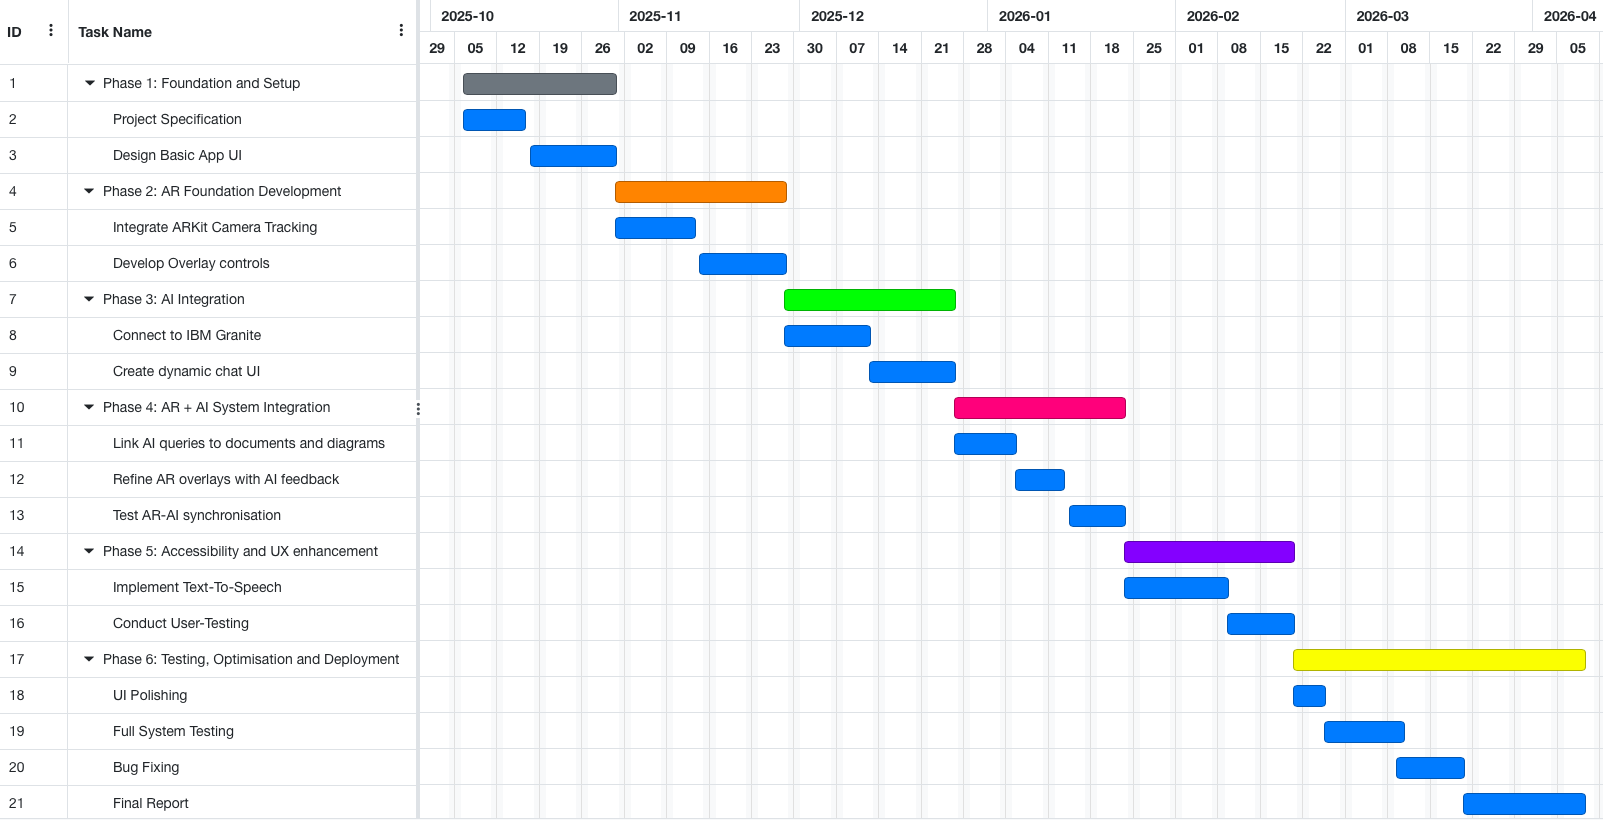
\includegraphics[width=\textwidth]{img/GanttChart.png}
        \caption{Gantt Chart of Planned Work Schedule}
        \label{fig:GanttChart}
        \end{figure}

\section{Resource Management}

    The project is primarily developed by a single developer, with support and guidance from the assessors. The developer is responsible for all aspects of the project, including design, implementation, testing and documentation.
    Access to the essential software tools and platforms, such as IBM Granite and IBM Cloud, are provided by IBM. Other resources, such as hardware for testing, necessary software and other materials, are handled by the developer. Except for the
    resources provided by IBM, the developer is responsible for acquiring any additional resources needed for the successful completion of the project. In the case of any type of resource unavailability, such as laptop malfunction or equipment failure, the
    developer will rely on the university's resources provided to students.


\section{Risk Management}
    The following risks have been identified for the project, along with their descriptions, risk levels, likelihoods and mitigation strategies.
        \begin{enumerate}
             
       
        \item{Technology Limitations}
        \begin{itemize}
            \item Risk description: There is unfamiliarity with some tools, libraries, or frameworks, which may cause delays or reduced performance. 
            \item Risk Level: Tolerable
            \item Risk Likelihood: Moderate
            \item Mitigation Strategy: Conduct thorough research and allocate time for learning and experimentation with new technologies.
        \end{itemize}

        \item{Rollback Challenges}
        \begin{itemize}
            \item Risk description: Lack of a version control system could prevent from rolling back to the software's last stable state in case of errors
            \item Risk Level: Catastrophic
            \item Risk Likelihood: Low
            \item Mitigation Strategy: Utilise GitHub to always maintain a stable version of the software and updating it when being sure that the changes will not affect its usability. 
        \end{itemize}

        \item{Testing Risks}
        \begin{itemize}
            \item Risk description: Insufficient testing may reduce confidence in the software
            \item Risk Level: Serious
            \item Risk Likelihood: Moderate
            \item Mitigation Strategy: Unit tests will be designed to test the software to make sure that it is working properly and user testing will be conducted to gather feedback and identify any issues.
        \end{itemize}

        \item{Time Management}
        \begin{itemize}
            \item Risk description: Underestimating  task duration or improper prioritization might result in delayed work.
            \item Risk Level: Serious
            \item Risk Likelihood: Low
            \item Mitigation Strategy: Meetings with the assessors will be held weekly to ensure that the project is on track and any issues are addressed promptly.
        \end{itemize}

        \item{Requirement Misalignment}
        \begin{itemize}
            \item Risk description: During the development of the software, the end product might not be the same as the one described in the deliverables due to unforeseen circumstances.
            \item Risk Level: Catastrophic
            \item Risk Likelihood: Low
            \item Mitigation Strategy: Regular meetings with the assessors will be held to ensure that the project is on track and any issues are addressed promptly.
        \end{itemize}

        \item{Underestimating Sprint Workload}
        \begin{itemize}
            \item Risk description: Tasks may take longer than expected due to AI and AR complexities, which may lead to incomplete sprints and delays.
            \item Risk Level: Serious
            \item Risk Likelihood: Moderate
            \item Mitigation Strategy: Buffer time will be allocated in each sprint to accommodate unforeseen challenges, and tasks will be prioritized to ensure critical features are completed first.
        \end{itemize}

        \end{enumerate}
        

\section{Legal, Social, Ethical and Professional Issues and Considerations}

    \subsection{Legal Issues}
        The project will comply with all relevant legal requirements, including data protection laws (e.g. UK GDPR), intellectual property rights and software licensing agreements. The application
        will not store any personal data without user consent, and all third-party libraries and tools used will be properly licensed and attributed. The developer will ensure that the application does not infringe on any patents or copyrights.

    \subsection{Social and Ethical Issues}
        As of now, there are no identified social or ethical issues related to the project. However, the developer will remain vigilant and address any concerns that may arise during the development process.

    \subsection{Professional Issues}
        The project will adhere to professional standards and best practices in software development, including code quality, documentation and testing. The developer will also ensure that the application is accessible to users with disabilities, following guidelines such as the Web Content Accessibility Guidelines (WCAG).
        
\section{Conclusion}

    In conclusion, this project aims to develop an application that uses Augmented Reality (AR) and Artificial Intelligence (AI) to help developers in understanding technical documentation better. By
    integrating AR overlays with an AI assistant, the application seeks to enhance the user experience, making complex technical concepts more accessible and easier to comprehend. The project will follow
    a structured development methodology, incorporating risk management strategies and adhering to legal, social, ethical and professional considerations. The successful completion of this project will result
    in a functional prototype that demonstrates the potential of combining AR and AI technologies to revolutionize the way technical documentation is presented and understood.

\end{document}